\begin{frame}{Induced fem in coil due to spinning M}
\begin{align*}
&emf=-\TDof{t}\int d^3r\vec{M}(\vec{r},t)\cdot\vec{\mathcal{B}}_{rec}\\
&S\propto \frac{\gamma^3B_0^2\rho_0}{T}
\end{align*}
\begin{figure}[!ht]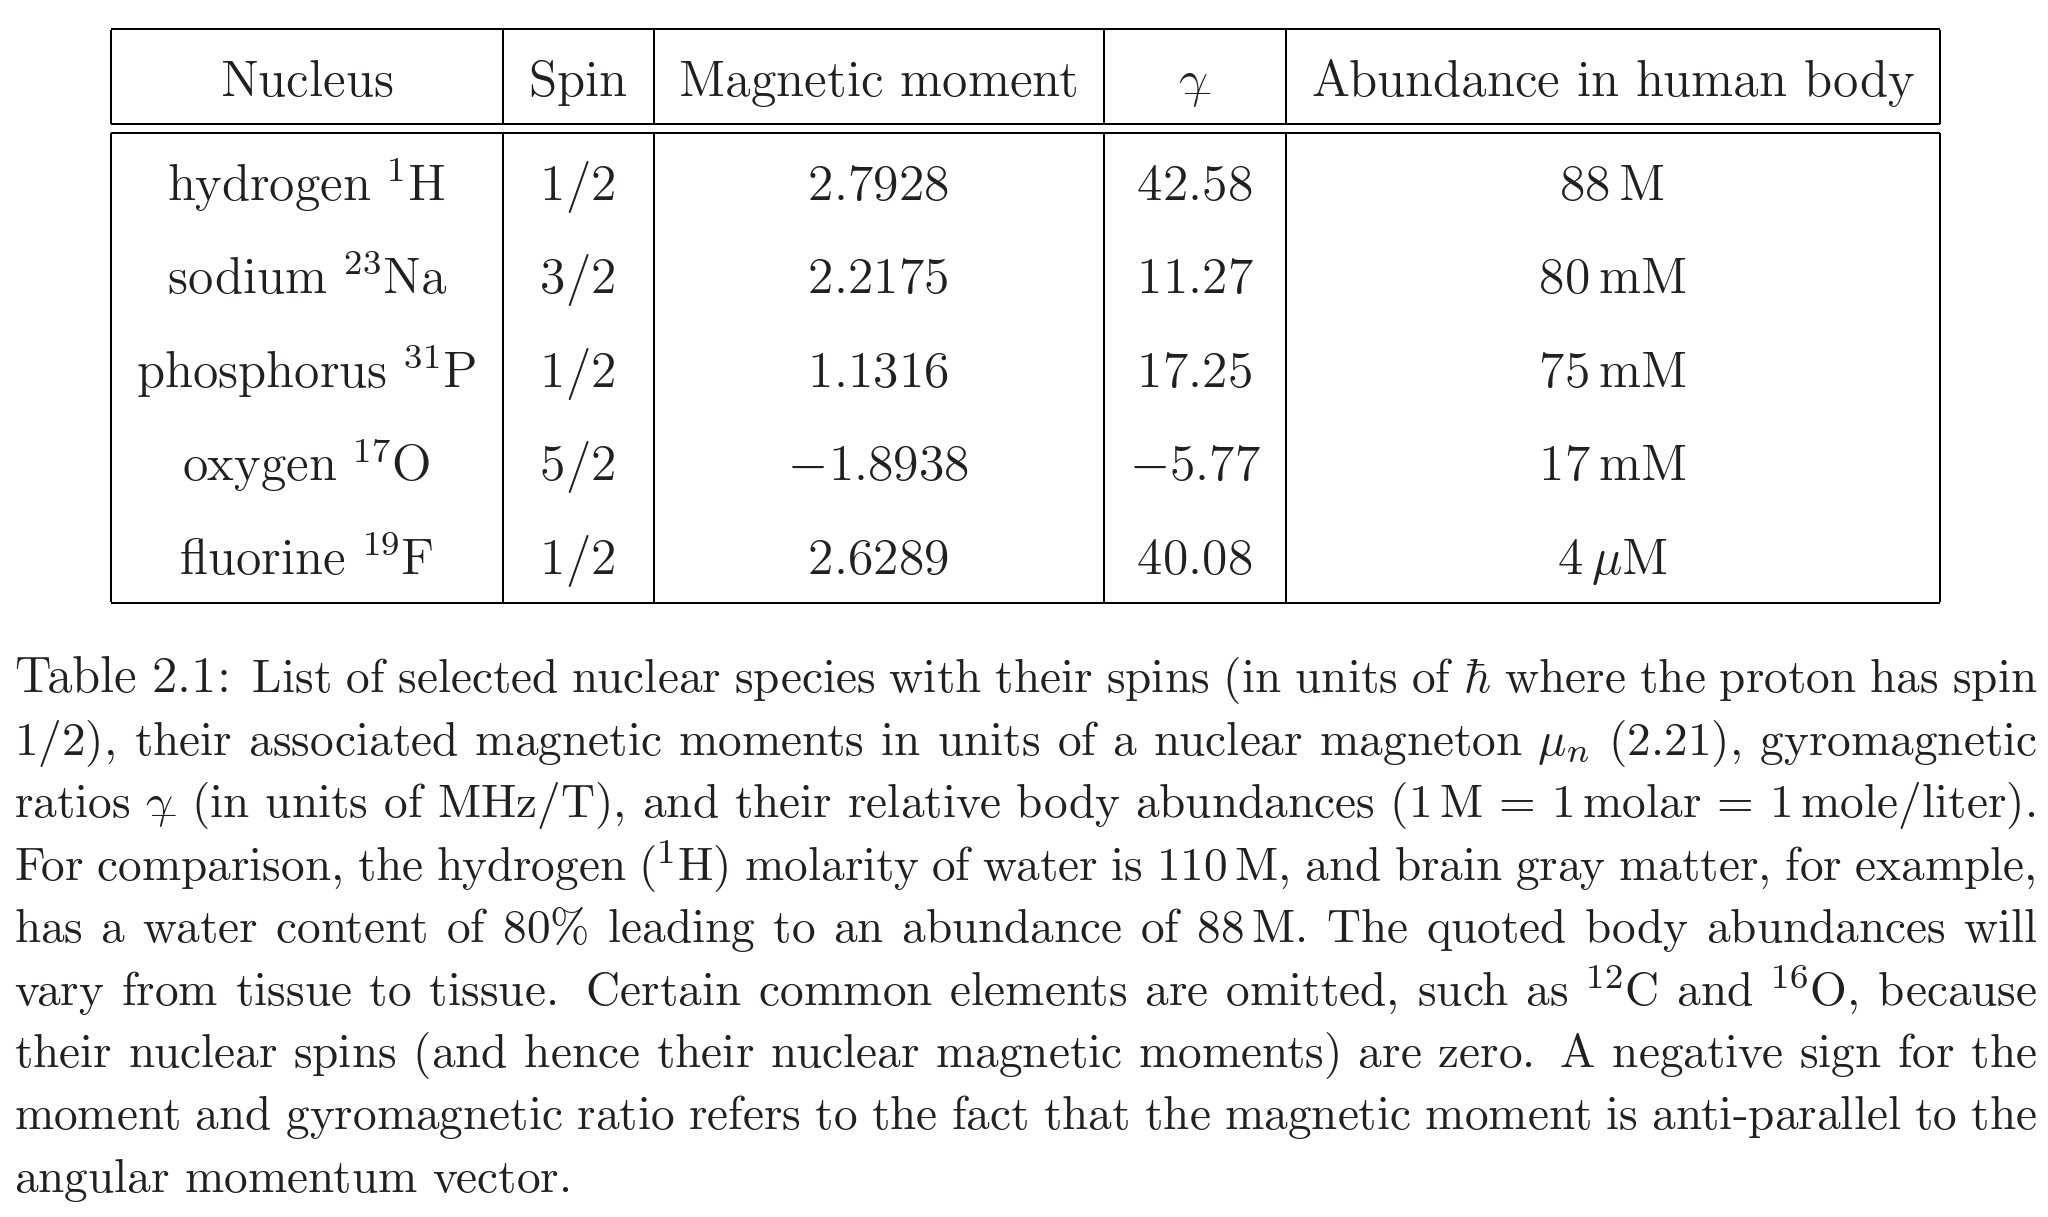
\includegraphics[trim={0cm 0cm 0 0},clip, keepaspectratio,width=0.5\textwidth]{nuclei}\label{fig:nuclei}\end{figure}
\end{frame}

\begin{frame}{On-resonance condition}
    Per $\omega=\omega_0$:
\begin{align*}
&(\TDy{t}{\vec{\mu}})'=\omega_1\vec{\mu}\wedge\hat{x}'
\end{align*}
Flip-angle: $\Delta\theta=\gamma B_1\tau$
\end{frame}

\begin{frame}{Equazione di Block}
$T_2*=T_2+T_2$: se domina $T_2'$ dovuto a disomogeneit\'a compo magnetico esterno $\magort{}$ pu\'o essere rifasata.
Interazioni spin-lattice: $T_1$.
\begin{align*}
&\TDy{t}{M_z}=\frac{(M_0-M_z)}{T_1}\\
&M_z(t)=M_z(0)\exp{-\frac{t}{T_1}}+M_0(1-\exp{-\frac{t}{T_1}})
\end{align*}
Local field variation: dephasing $T_2$.
\begin{align*}
&\TDy{t}{\magort}=(\gamma\magort{}\wedge\vec{B}_{ext})_{NR}-\frac{1}{T_2}\magort{}\\
&\magort{}(t)=\magort{}(0)\exp{-\frac{t}{T_2}}
\end{align*}
\end{frame}

\begin{wordonframe}{Magnetismo elettronico}
La maggior parte delle molecole hanno stato fondamentale elettronico $S=L=0$: no momento magnetico. Eccezioni: $\cel{O}{2}{}{}$ con stato fondamentale $S=1$, composti con metalli di transizione, molecole con elettroni dispari.
La maggior parte dei composti sono diamagnetici ($\chi<0$: weak diamagnetis induced by electron orbital current).
Sostanza con momento magnetico in stato fondamentale sono solitamente paramagnetiche ($\chi>0$): se electron magnetic moment interagiscono debolmente \'e possibile EPR-ESR.
(NMR in diamagnetic material: electron magnetism can be ignored because is constant, correzione a campo staticoi)
\end{wordonframe}

\begin{wordonframe}{Kubo: fluctuatuion-dissipation theorem}

\end{wordonframe}

\begin{wordonframe}{Real spectrum FFT: 34-49}
Lorentzian shape-inhomogeneous field broadening-chemical shift(diamagnetic)/spin-spin coupling-J coupling
\end{wordonframe}

\begin{wordonframe}{processi rilassamento spin-spin, spin-lattice}
Lewitt (S dyn): 171-190 nuclear interaction with electric magnetic field (Spin hamiltonian), 543-624 types of relaxation: mechanism, random field relaxation, spectral density, transition probability (dipole-dipole relaxaion: solomon equation, neclear overhauser effectà-)
\end{wordonframe}

\begin{wordonframe}{Nuclear spin interactions}
Spin hamiltonian hypothesis: fast electron motion, low nuclear spin energy.
Nuclear shape, rotation: change in electric/magnetic energies due to orientatio changes.
\end{wordonframe}

\begin{frame}[allowframebreaks]{Free induction decay}

$\pi/2$ pulse lungo $x'$:
\begin{align*}
s(t)\propto\omega_0\int d^3r \exp{-\frac{t}{T_{2}(r)}}B_{\perp}(\vec{r})M_{\perp}(\vec{r},0)\exp{i[(\Omega-\omega(r))t+\phi_0(\vec{r})+\theta_B(\vec{r})]}\\
\phi(\vec{r},t)=-\omega(r)t+\phi_0(\vec{r})=-\gamma B_z(\vec{r})t+\phi_0(\vec{r})
\end{align*}
\begin{figure}[!ht]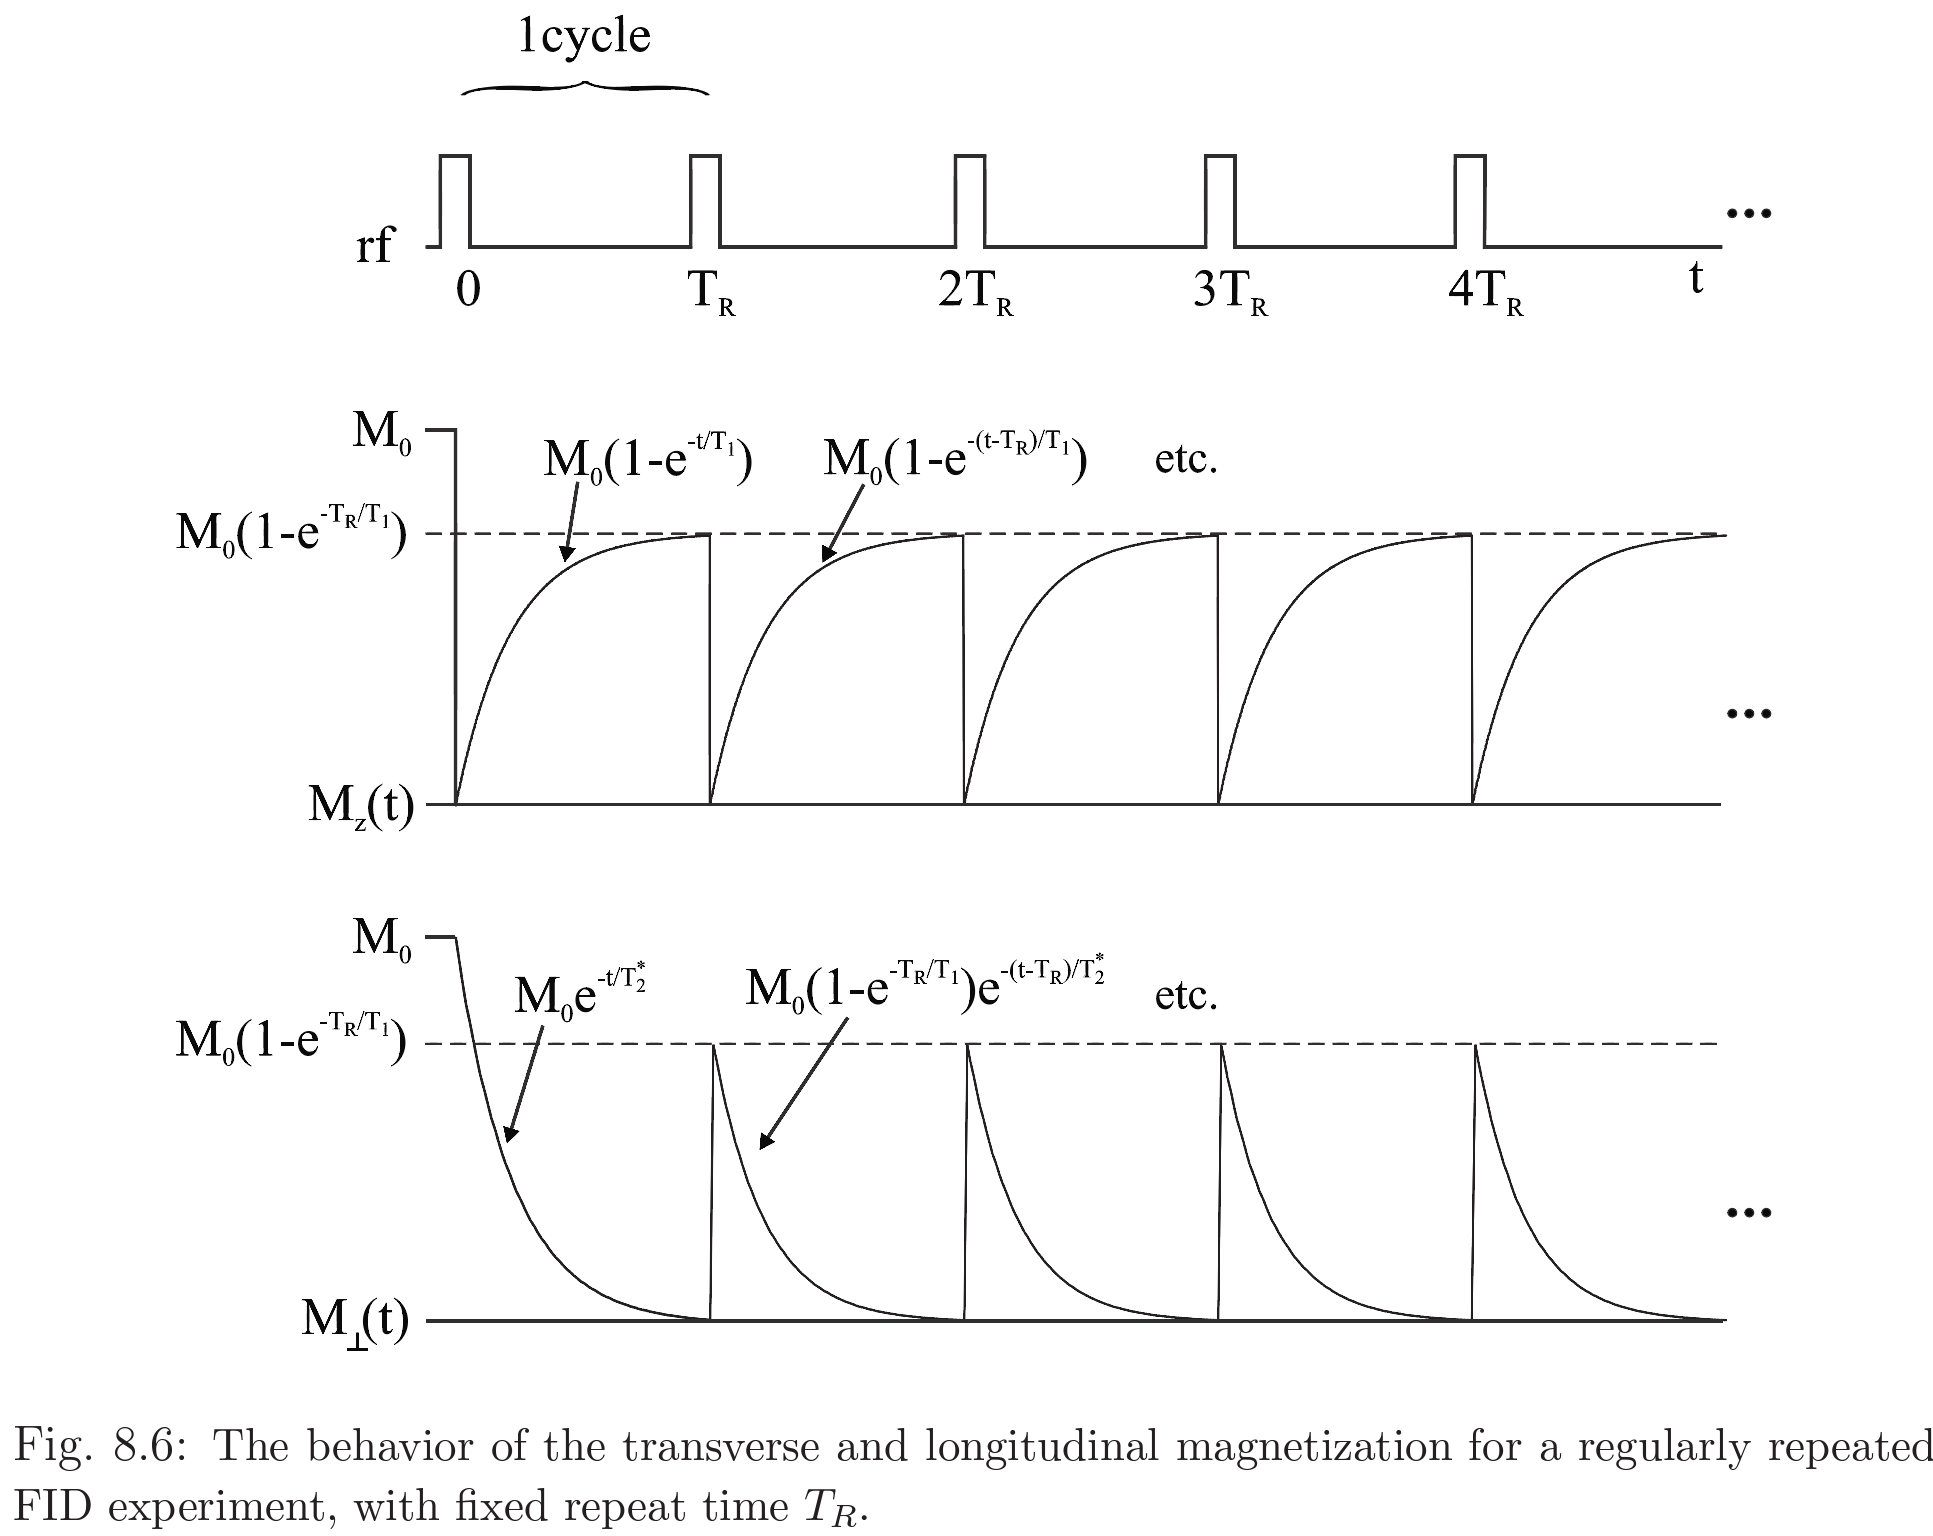
\includegraphics[trim={0cm 0cm 0 0},clip, keepaspectratio,width=0.4\textwidth]{FIDrep}\label{fig:FIDrep}\end{figure}
\begin{align*}
\frac{1}{T_2*}=\frac{1}{T_2}+\frac{1}{T_2'}\\
M_+(\vec{r},t)=M_+(\vec{r},0)\exp{-\frac{t}{T_2*}}\\
\phi(\vec{r},t)=-\gamma[B_0+\Delta B(\vec{r})]t
\end{align*}
\end{frame}

\begin{frame}[allowframebreaks]{Spin-ECHO and $T_2$ measure.}

\begin{figure}[!ht]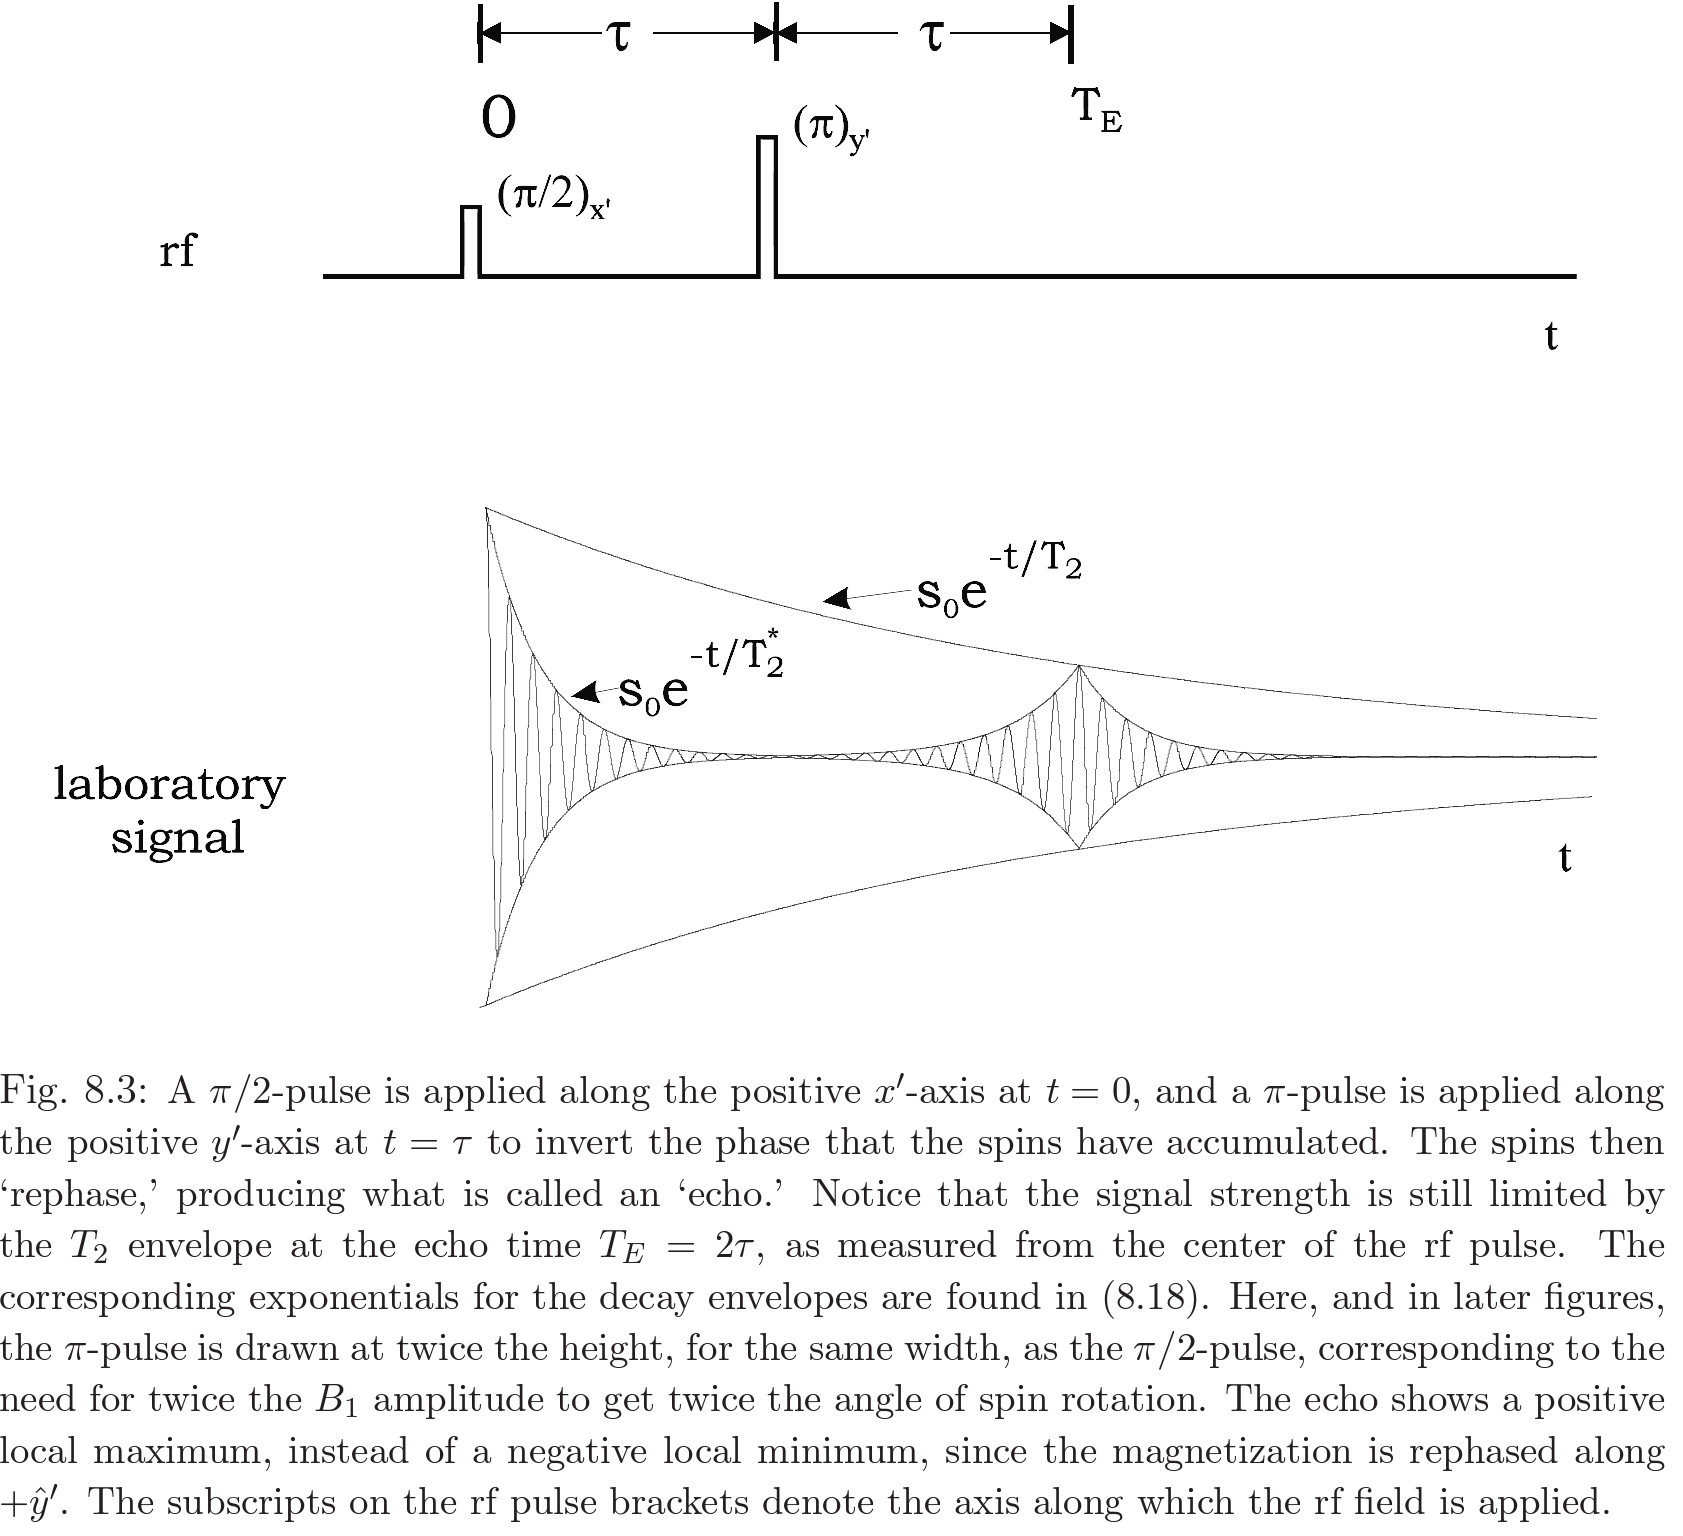
\includegraphics[trim={0cm 0cm 0 0},clip, keepaspectratio,width=0.5\textwidth]{SE}\label{fig:SE}\end{figure}
\begin{figure}[!ht]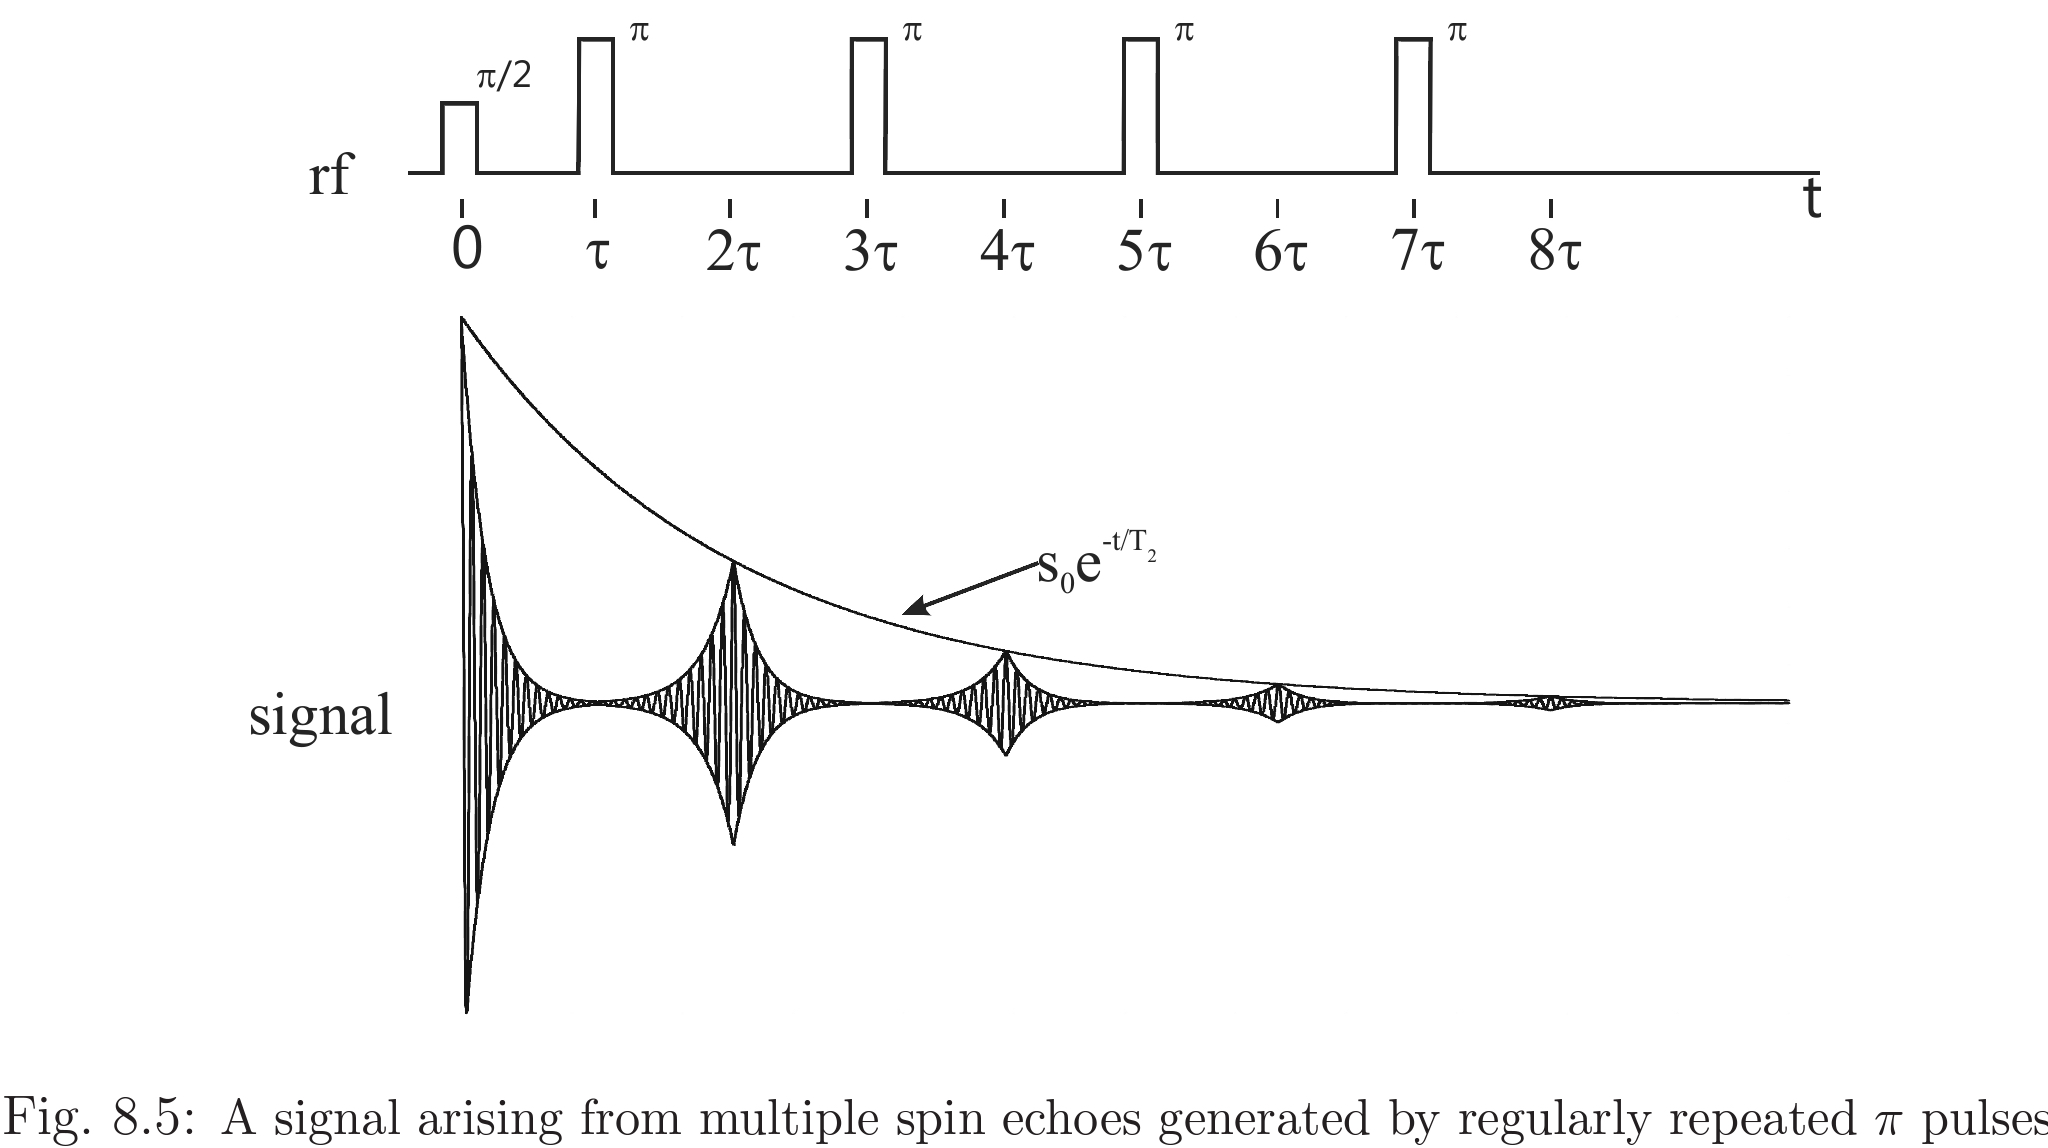
\includegraphics[trim={0cm 0cm 0 0},clip, keepaspectratio,width=\textwidth]{SET2measure}\label{fig:SET2measure}\end{figure}
\begin{align*}
s(T_E)\propto\omega_0\exp{-\frac{T_E}{T_2}}\int d^3 rB_{\perp}M_{\perp}(\vec{r},0)\\
T_2=\frac{T_E'-T_E}{\ln{[s(T_E)/s(T_E')]}}
\end{align*}
\end{frame}

\begin{frame}[allowframebreaks]{Inversion recovery and $T_1$ measure - Spin-echo inversion recovery.}
%succo
Impulso $\pi$ attorno $x'$ e a $T_I$ di $\pi/2$
\begin{align*}
&M_z(0+)=-M_0\\
&M_z(t)=-M_0\exp{-\frac{t}{T_1}}+M_0(1-\exp{-\frac{t}{T_1}})\ 0<t<T_I\\
&\magort{}(t)=|M_0(1-2\exp{-\frac{T_I}{T_1}})|\exp{-\frac{(t-T_I)}{T_2*}}\\
&T_I^{null}=T_1\ln{2}
\end{align*}

\begin{figure}[!ht]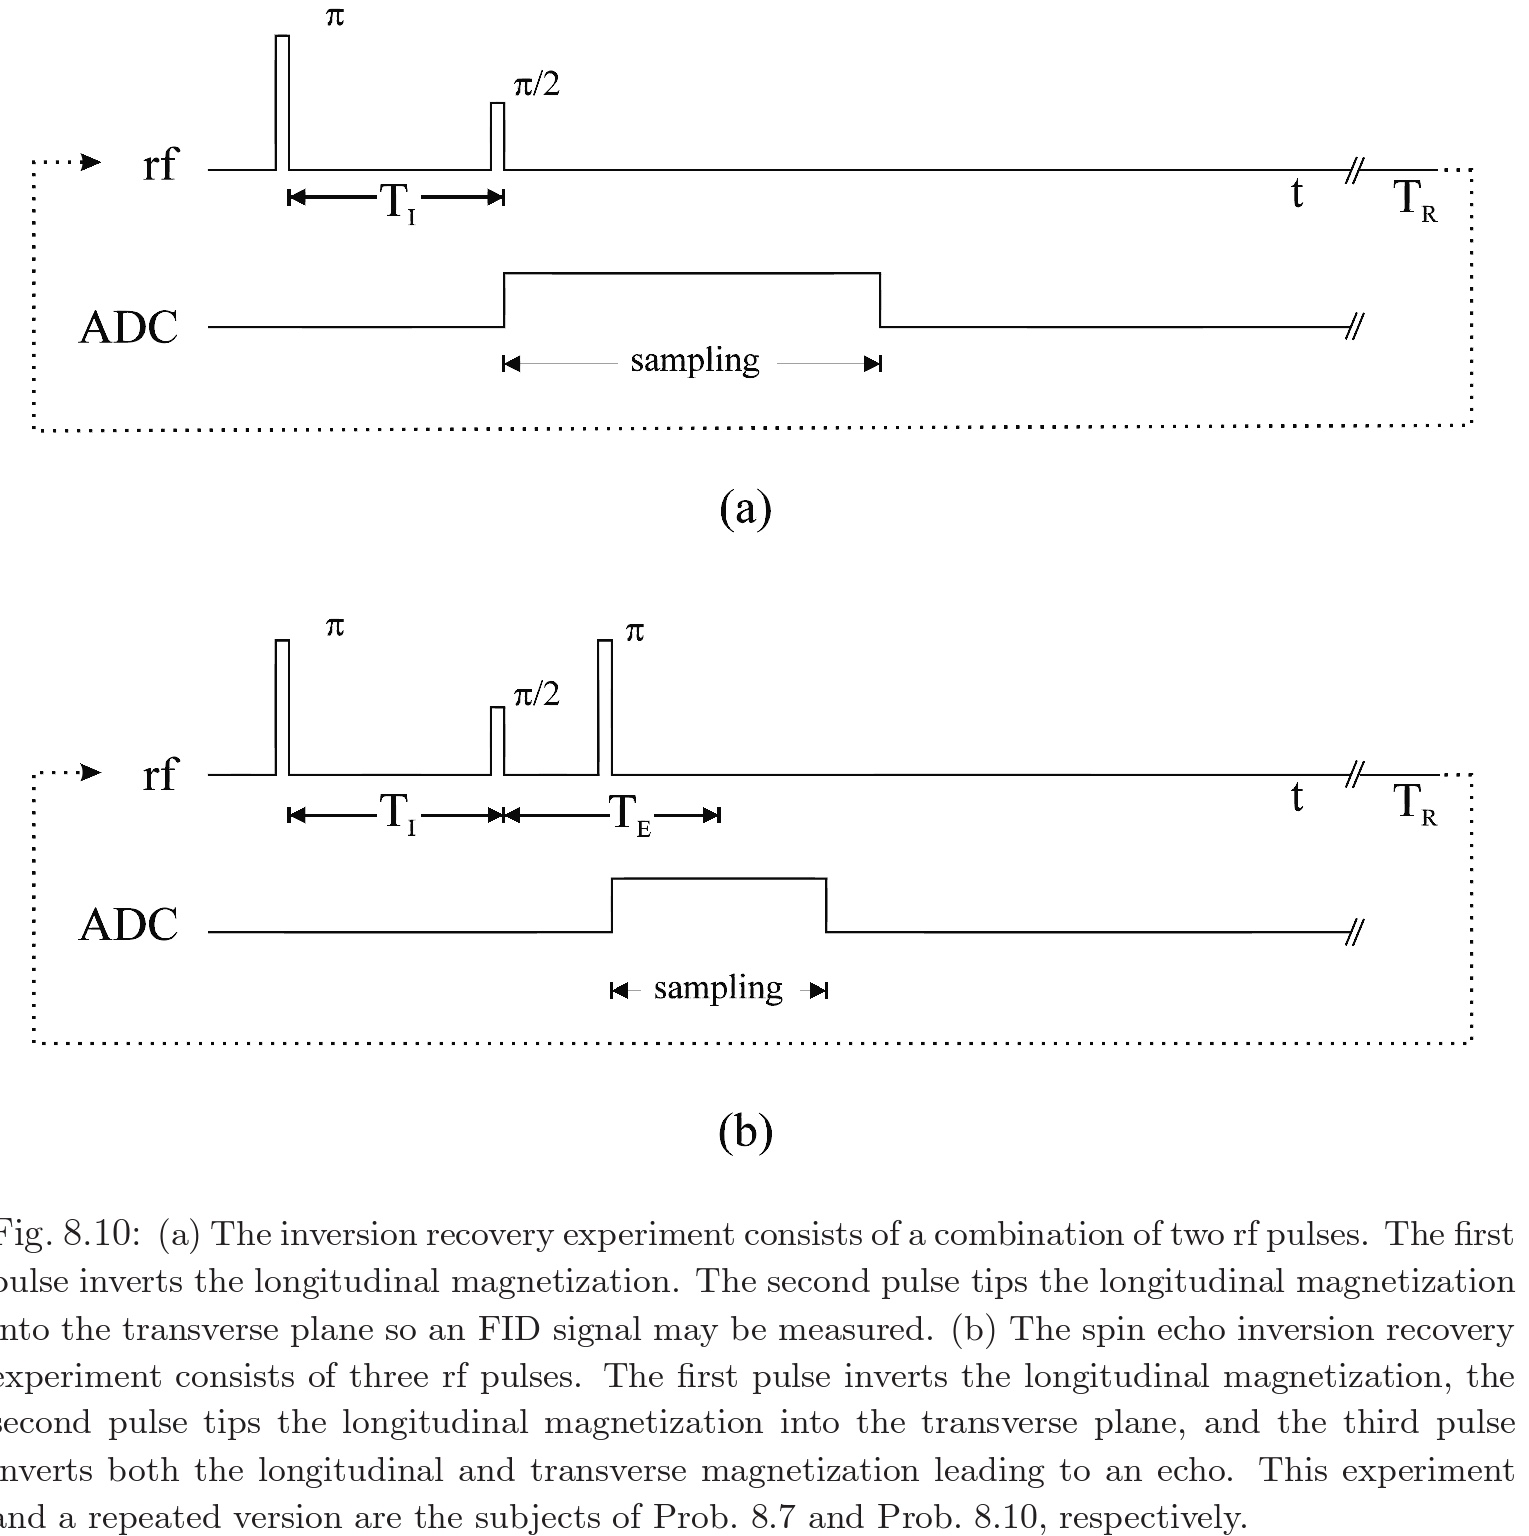
\includegraphics[trim={0cm 0 0 0},clip, width=0.9\textwidth]{IR-SE-sampling}\label{fig:IR-SE-sampling}
\end{figure}

\begin{figure}[!ht]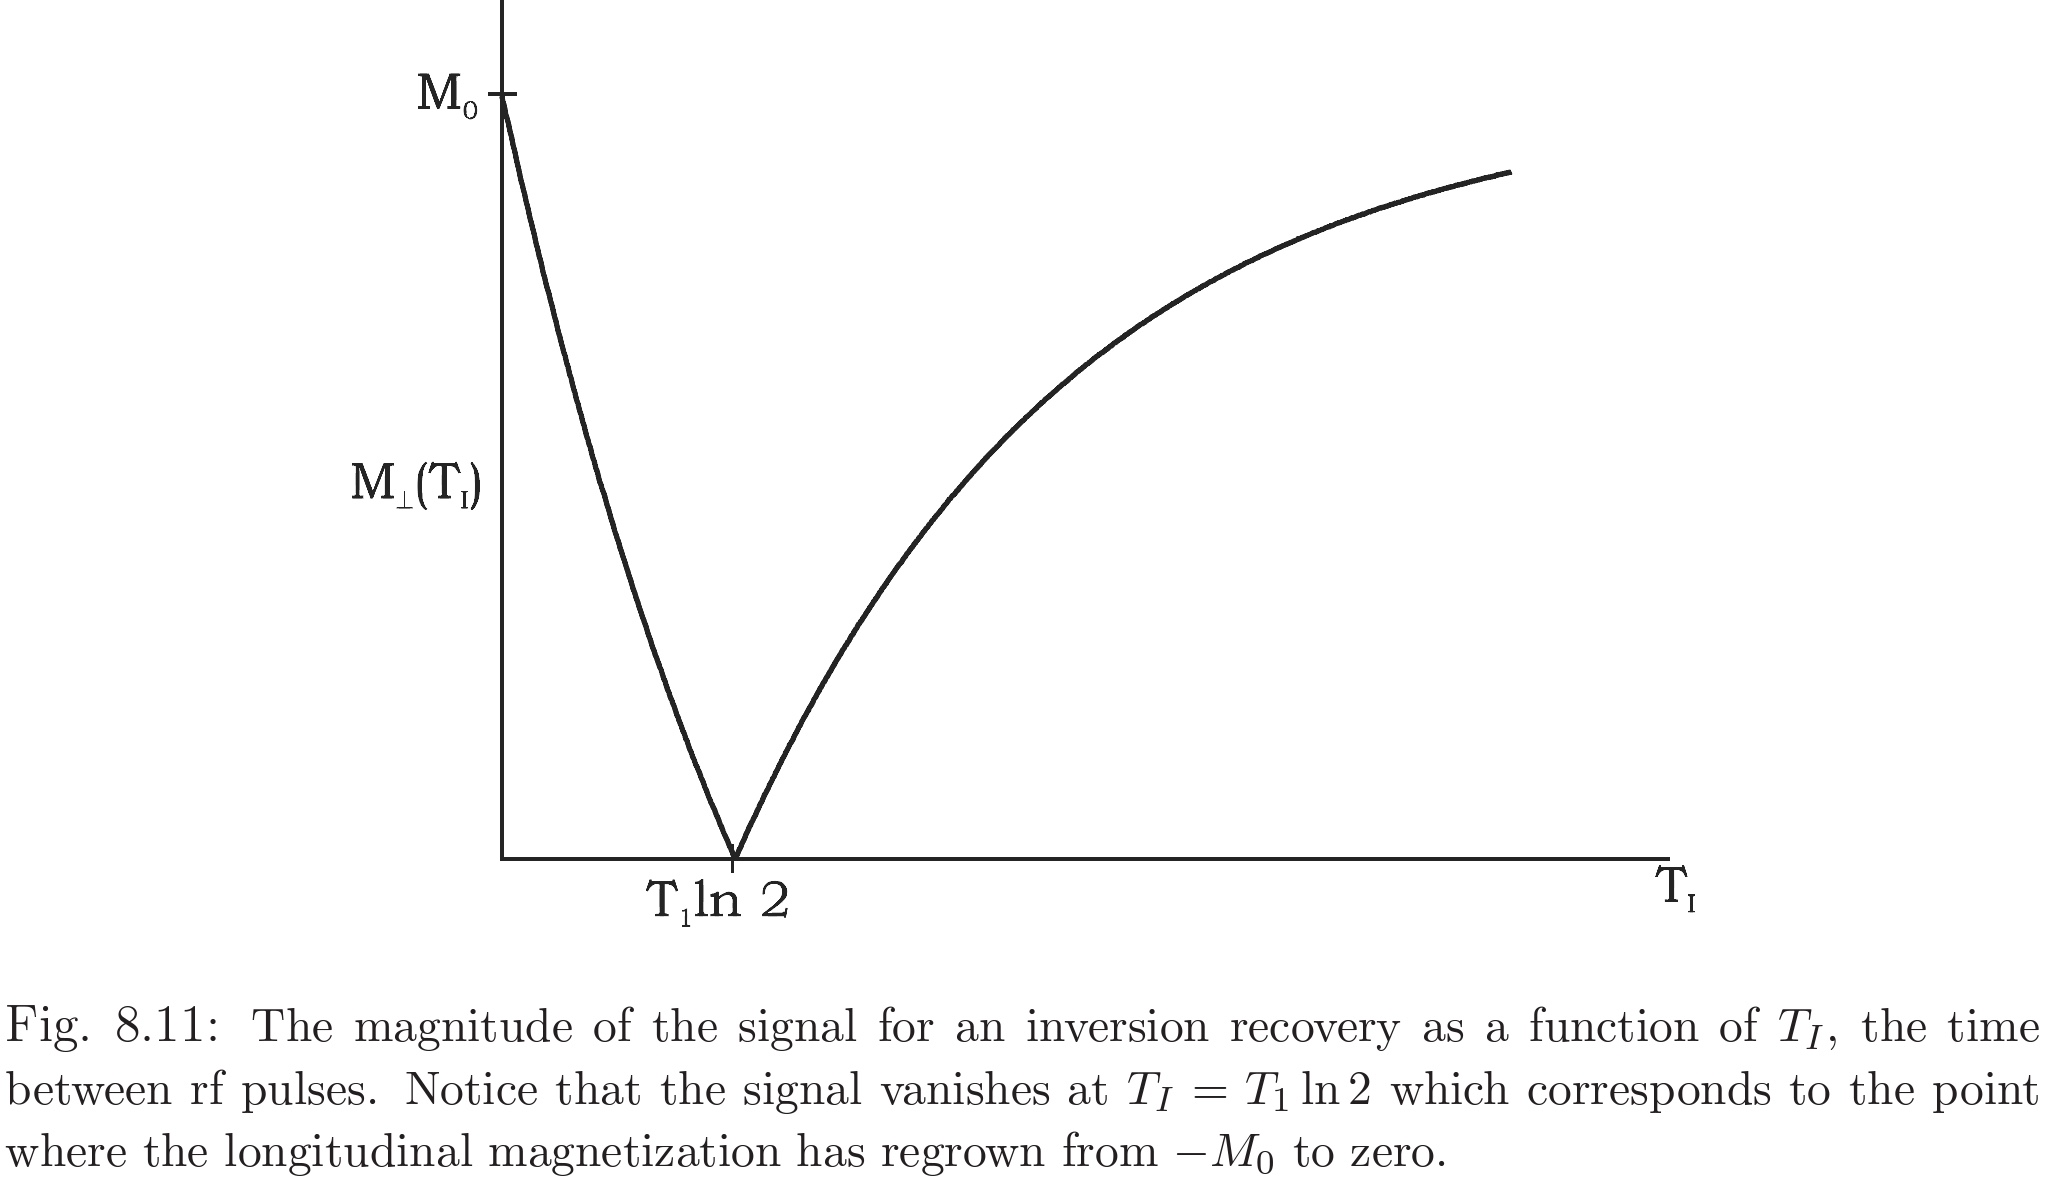
\includegraphics[trim={0cm 0 0 0},clip,width=0.9\textwidth]{IRvsTI}\label{fig:IRvsTI}\end{figure}

\end{frame}

\begin{frame}{Chemical shift and NMR spectroscopy}

Broadband RF excitation: complicated FID signal
\begin{align*}
&\omega_{0i}=\gamma_iB_0\\
&\vec{B}_j^{ind}=\delta_j\vec{B}_0
\end{align*}

Shielding constant: linear response of electrons to $B_{ext}$:
\begin{align*}
&B_{shift}(j)=(1-\sigma_j)B_0\to f_{\sigma}=-\sigma\gammabar B_0\\
&s(t)=\sum_jN_j\exp{i\gamma\sigma_jB_0t}
\end{align*}
\end{frame}


\begin{frame}{Fourier imaging}
Aggiungo campo che varia linearmente lungo z:

\begin{align*}
&s(t)\propto\int d^3 r\rho(\vec{r})\exp{i[\Omega t+\phi(\vec{r},t)]}\\
&B_z(z,t)=B_0+zG(t)\ \Rightarrow\ \omega=\omega_0+\omega_G(z,t)
\end{align*}

Frequency encoding: $\omega_G=\gamma zG(t)$.
\begin{equation*}
\phi_G(z,t)=-\int_0^td t'\omega_G(z,t')=-\gamma z\int_0^td t'G(t)
\end{equation*}

1D imaging equation (after demodulation):
\begin{align*}
&s(t)=\int d z\rho(z)\exp{i\phi_G(z,t)}\to s(k)=\int d\,z\rho(z)\exp{-i2\pi kz}\\
&\rho(z)=\int d\,ks(k)\exp{i2\pi kz}
\end{align*}
$\rho$ effective spin density.

\end{frame}

\begin{frame}{Gradient echo}
\begin{figure}[!ht]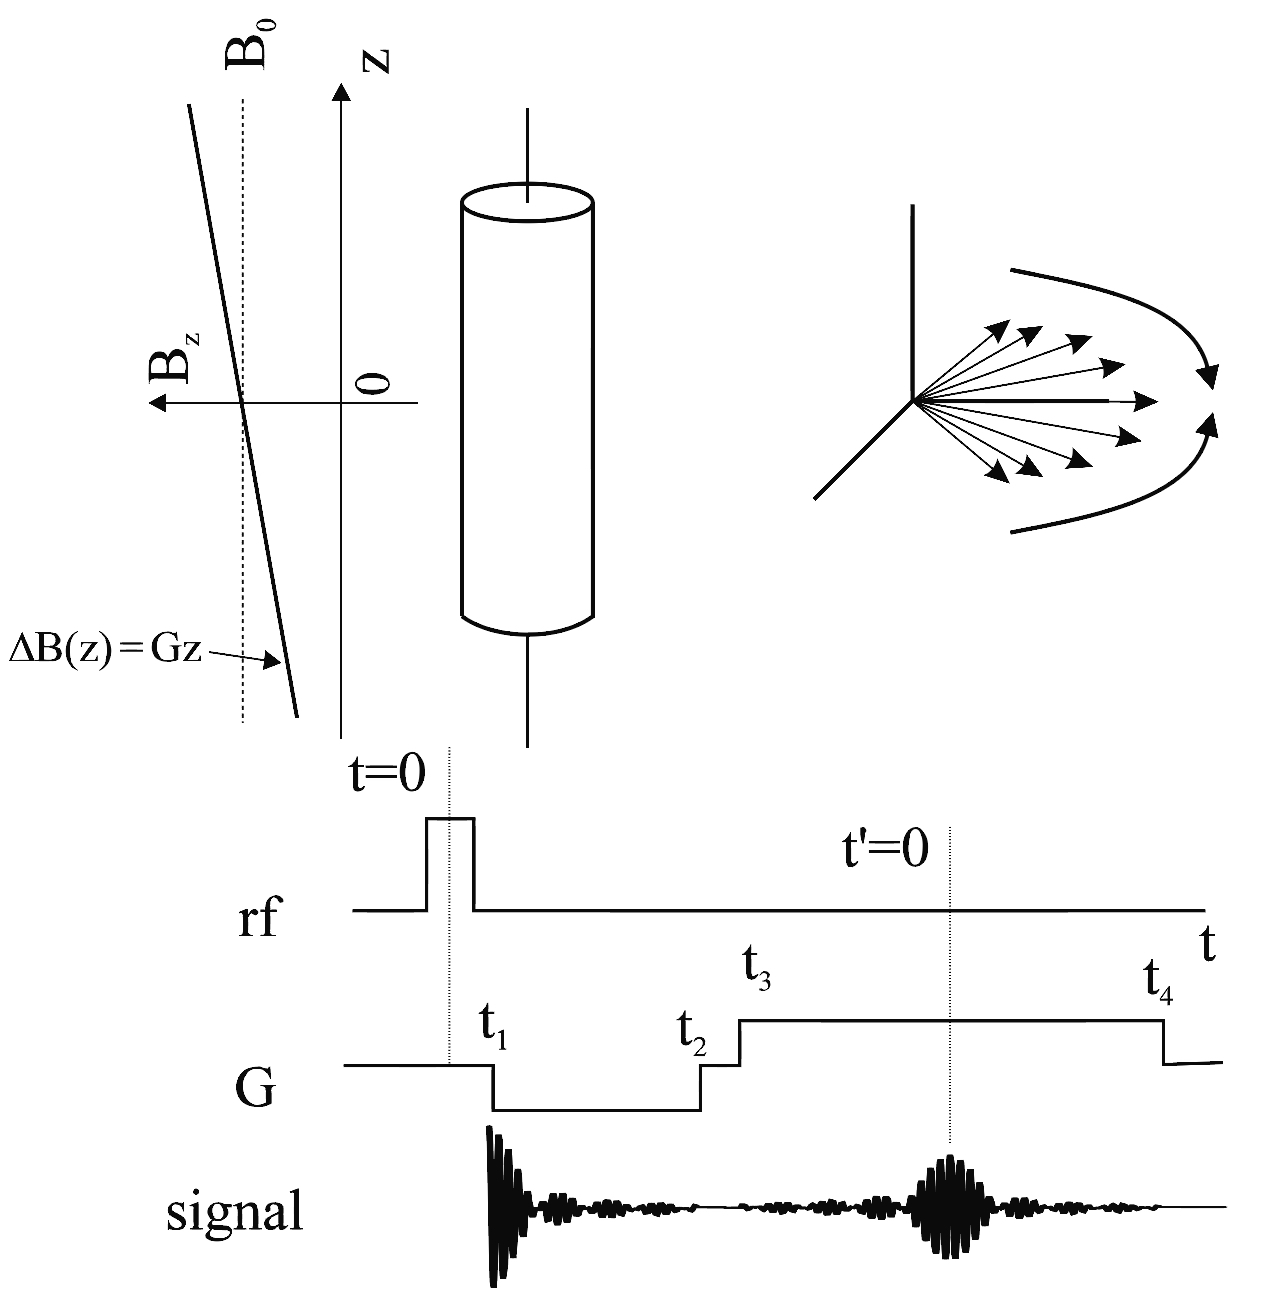
\includegraphics[trim={0cm 0cm 0 0},clip, keepaspectratio,height=0.9\textheight]{GEimaging}\end{figure}
\end{frame}

\begin{frame}[allowframebreaks]{Spin-echo imaging}
\begin{figure}[!ht]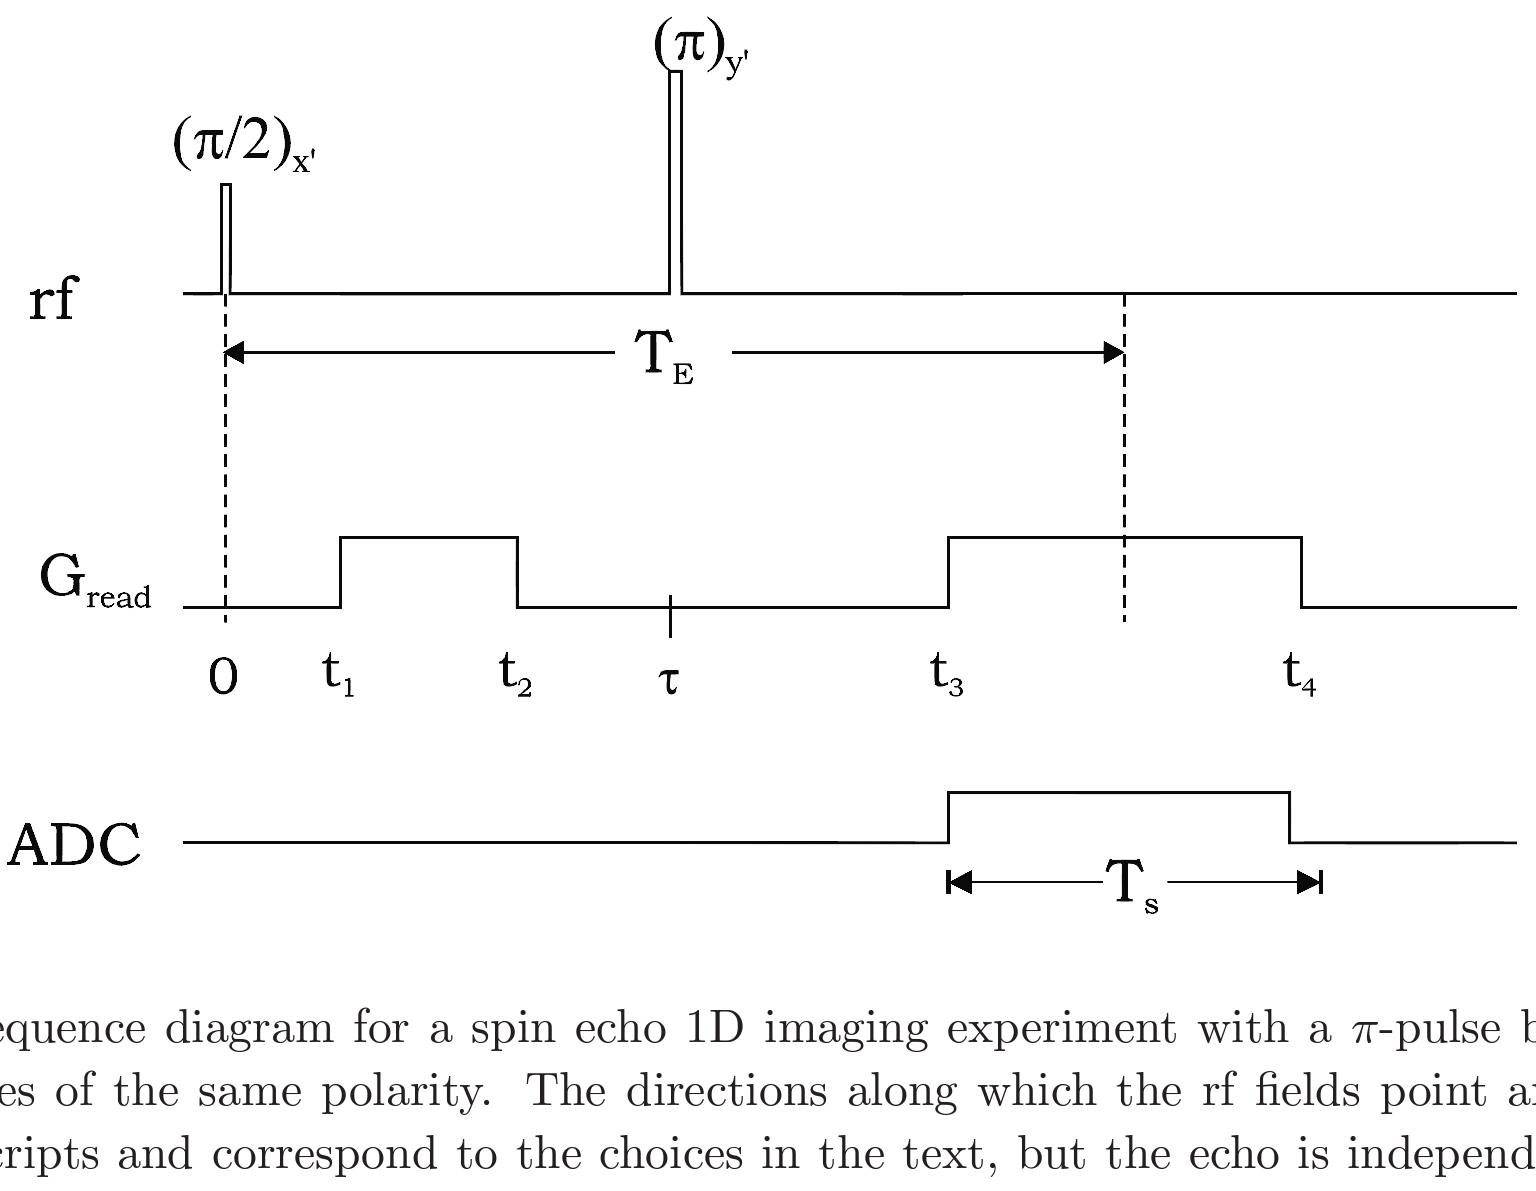
\includegraphics[trim={0cm 0cm 0 0},clip, keepaspectratio,height=0.45\textheight]{SEimaging}\end{figure}
\begin{figure}[!ht]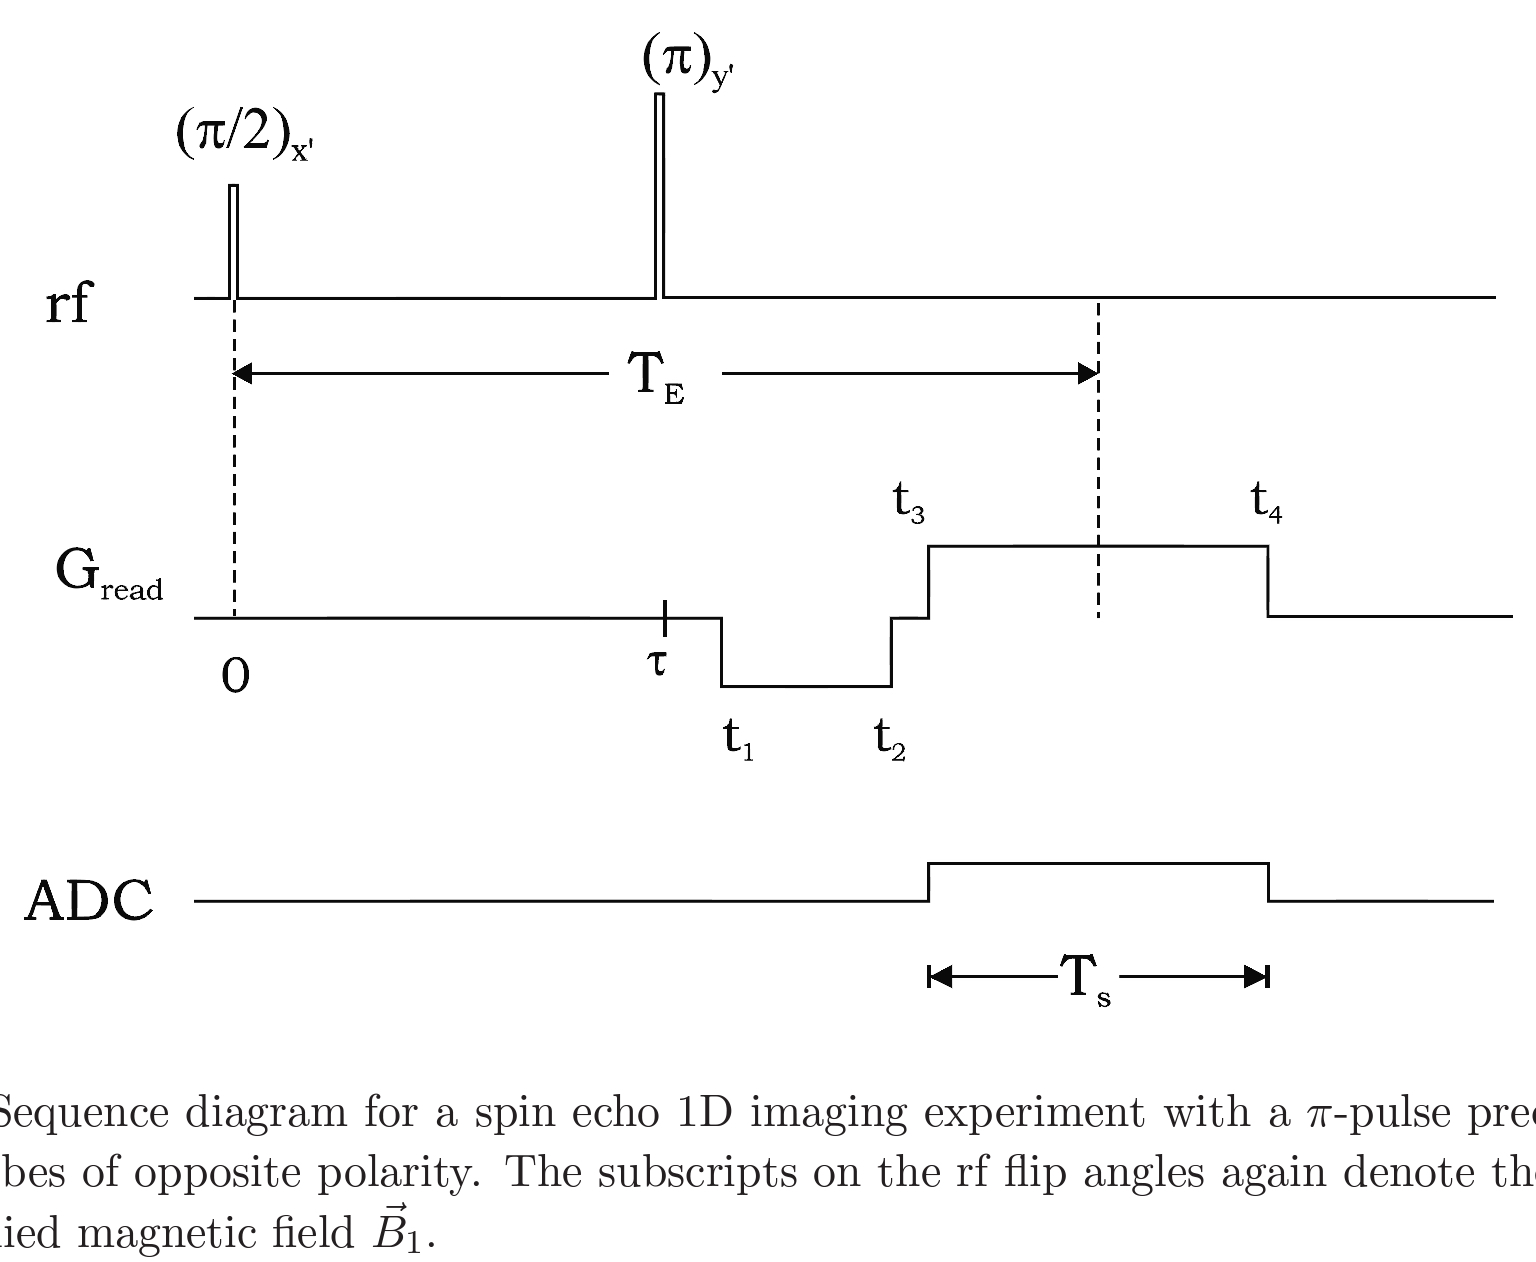
\includegraphics[trim={0cm 0cm 0 0},clip, keepaspectratio,height=0.45\textheight]{SEtotimaging}\end{figure}
\end{frame}

\begin{frame}[allowframebreaks]{Imaging in 3D: 3D imaging  vs 2D multislice imaging}
\begin{columns}[T]
\begin{column}{0.5\textwidth}
3D imaging:
\begin{figure}[!ht]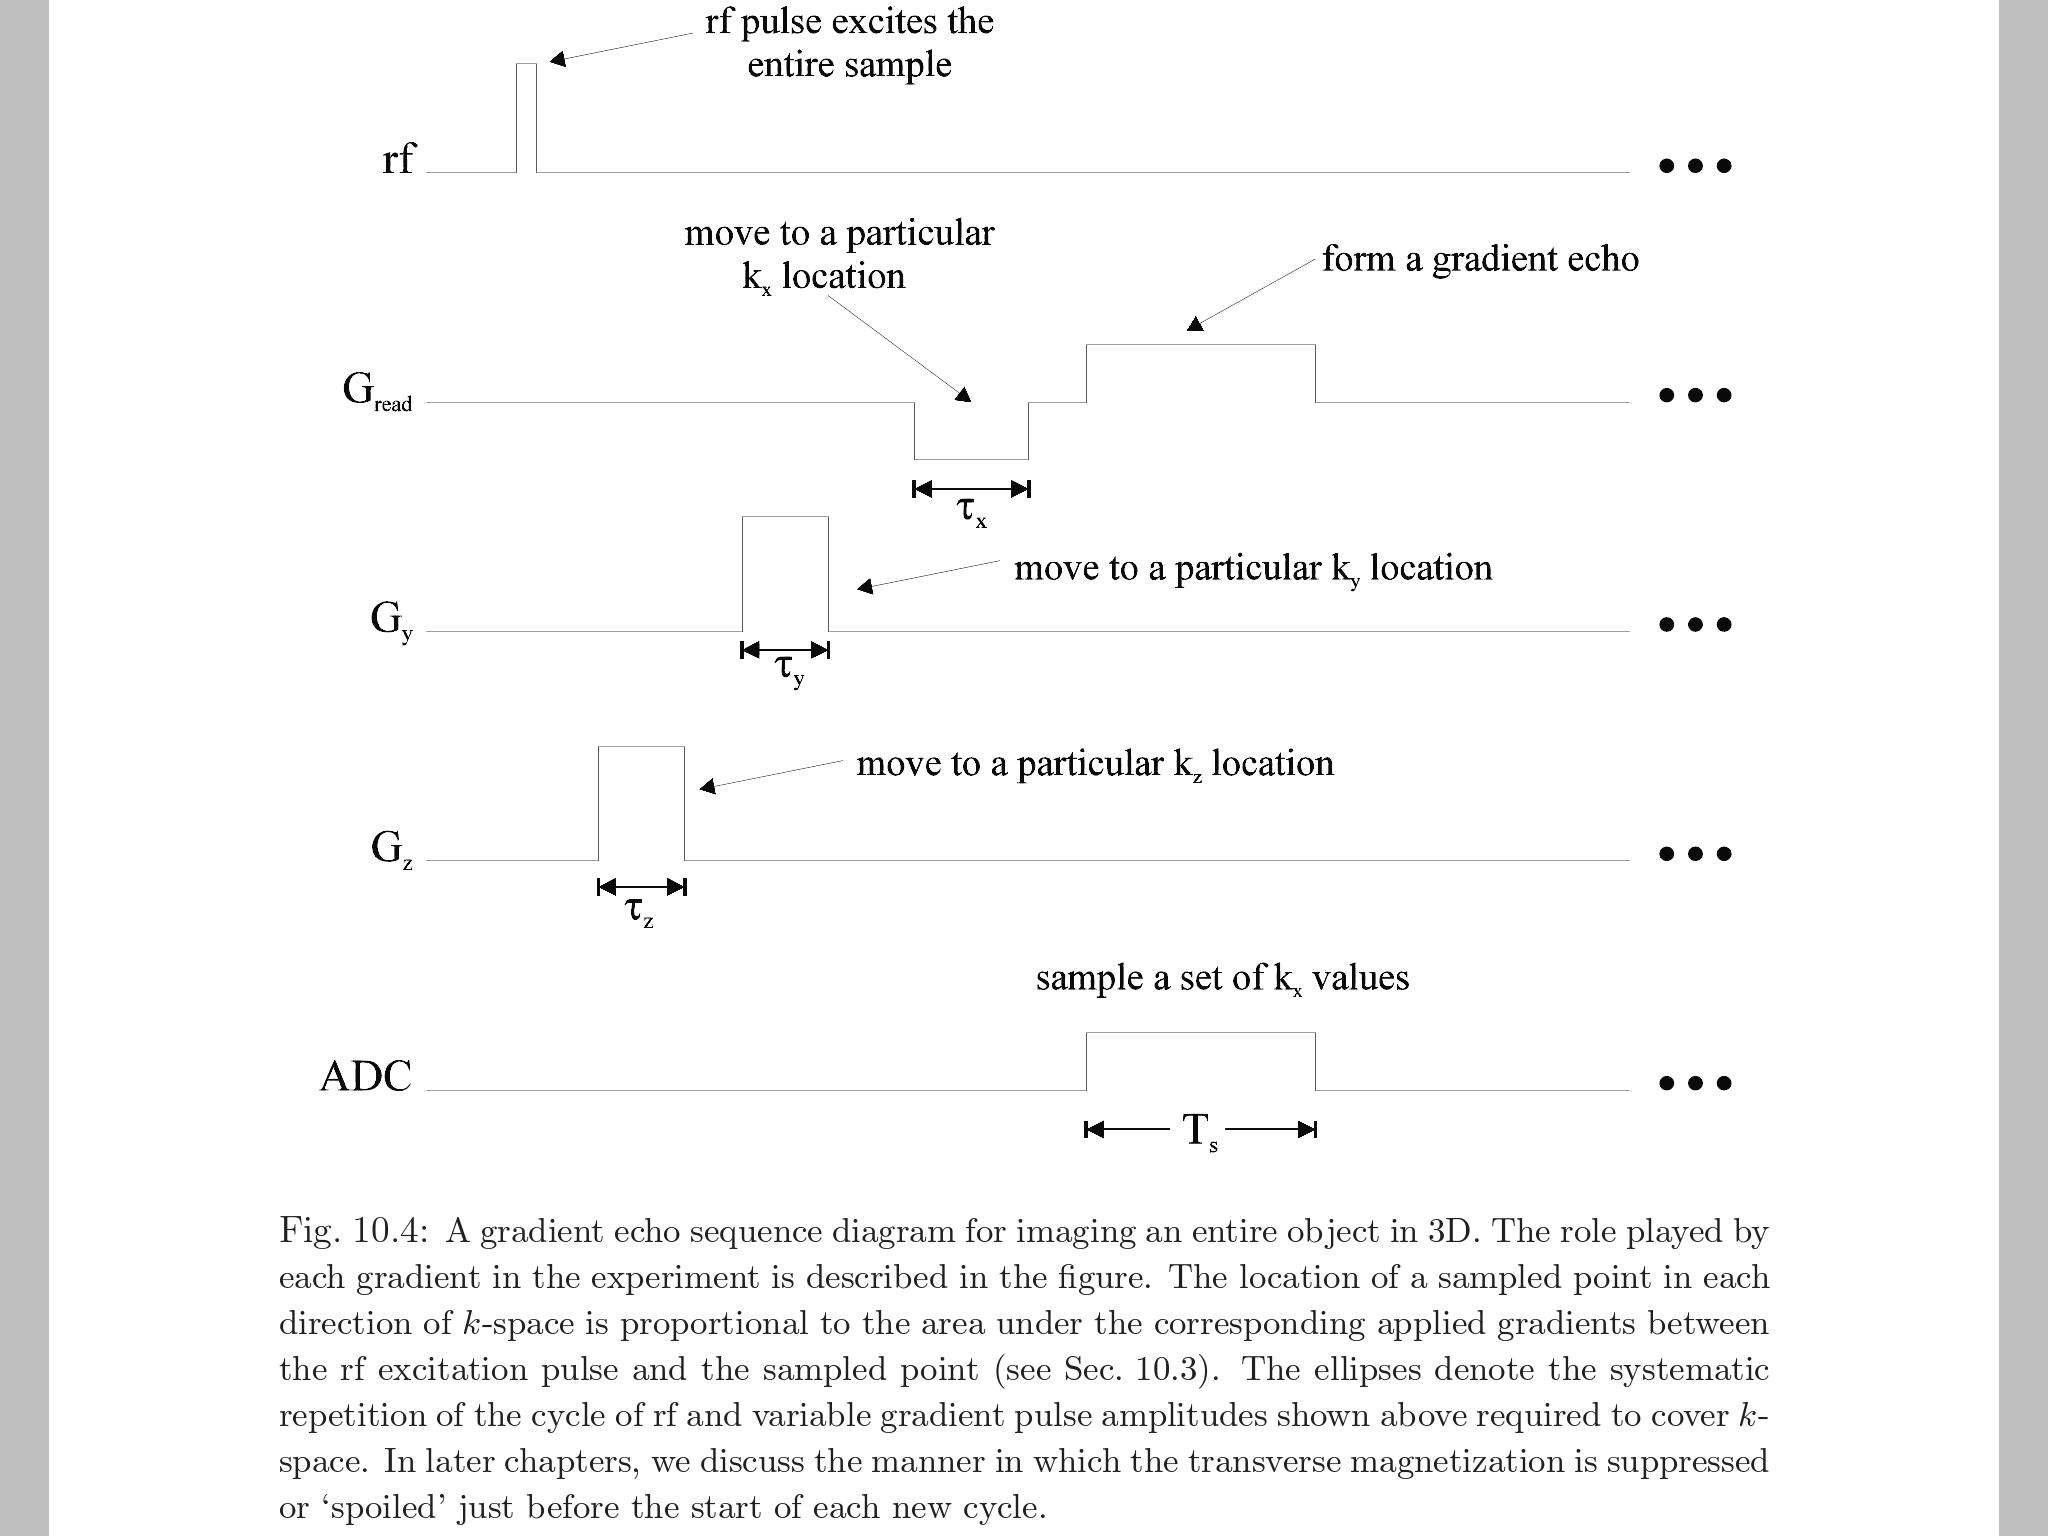
\includegraphics[trim={5cm 0cm 5cm 0},clip, keepaspectratio,width=0.99\textwidth]{3Dimaging}\label{fig:3Dimaging}\end{figure}
\end{column}
\begin{column}{0.49\textwidth}
2D multi-slice imaging:
\begin{figure}[!ht]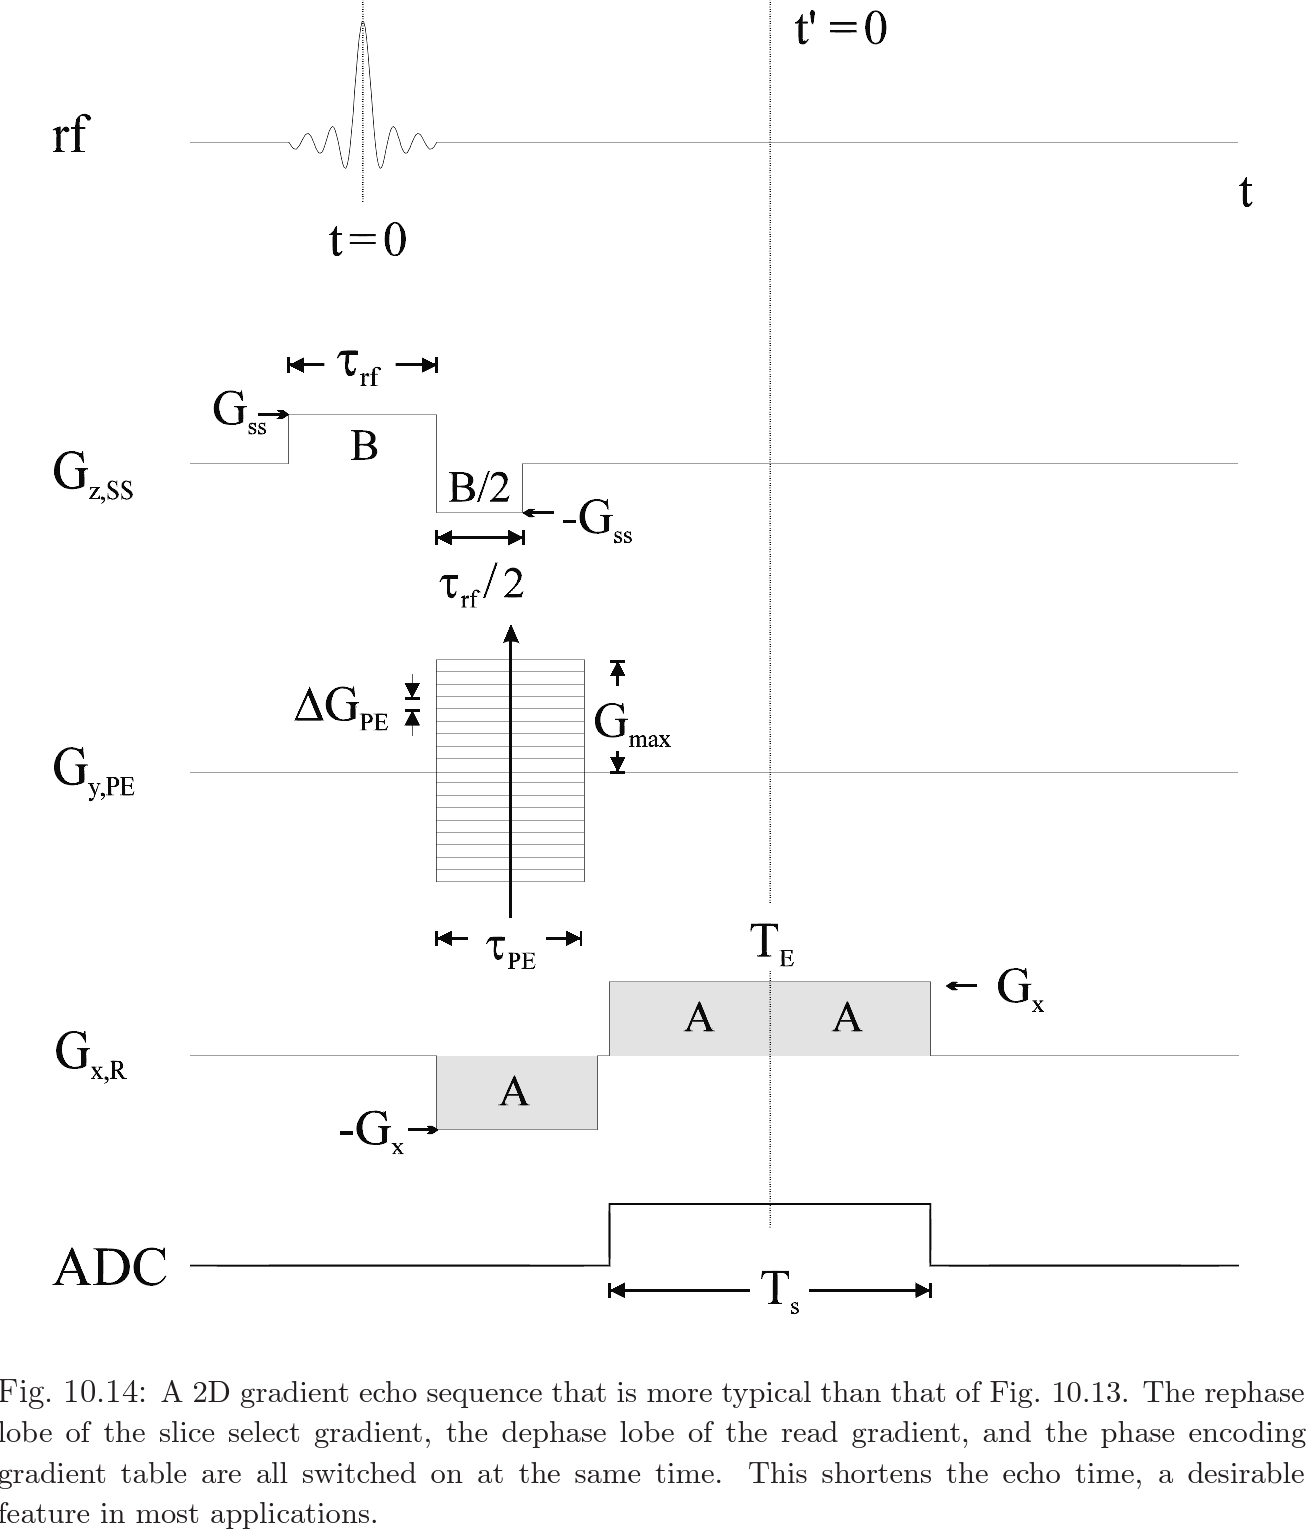
\includegraphics[trim={0cm 0cm 0 0},clip, keepaspectratio,width=0.99\textwidth]{sliceselection}\label{fig:sliceselection}\end{figure}
\end{column}
\end{columns}
\end{frame}

\begin{frame}[allowframebreaks]{Nyquist criterion, resolution and contrast}
\begin{align*}
&(FOV)^{-1}=\Delta k<\frac{1}{A}\\
&(\Delta k_R=\gammabar\int_t^{t+\Delta t}d t'G_R(t')=\frac{1}{L_R}<\frac{1}{A_R})\\
&f_R=BW_{read}=\frac{1}{\Delta t}=\gammabar G_RL_R>\gammabar G_RA_R
\end{align*}
Risoluzione: $\Delta x=\frac{1}{2n\Delta k}$, $k=(-n\Delta k,(n-1)\Delta k)$.

\begin{align*}
&\SNR/Vxl\propto\frac{\sqrt{N_{aqr}}}{\sigma_0}\quad \Delta t= \frac{1}{\BW_{read}},\ T_s=N_x\Delta t\\
&\SNR/Vxl\propto \frac{\Delta x\Delta y\Delta z\sqrt{N_a}}{\BW_{read}/(N_xN_yN_z)}
\end{align*}
Degrading resolution to improve SNR.

\begin{align*}
&C_{AB}=S_A-S_B\\
&=\rho_{0A}(1-\exp{-\frac{T_R}{T_{1A}}})\exp{-\frac{T_E}{T*_{2A}}}-\rho_{0B}(1-\exp{-\frac{T_R}{T_{1B}}})\exp{-\frac{T_E}{T*_{2B}}}
\end{align*}
Weighting
\end{frame}